\section{The Emergence of Heterogeneous Computing}

    For several decades, from the 1970s until the early 2000s, advances in
    processor development followed Moore's Law \citep{4785860} and
    Dennard Scaling \citep{1050511}.
    The density of integrated circuits doubled every two years,
    and this allowed increased clock frequencies while maintaining
    steady power consumption.
    These conditions enabled continual processor improvements that were driven
    primarily by rising clock frequencies and microarchitectural refinements,
    enabling ever faster computations.

    The physics-driven nature \citep{Hutcheson2018Moore} of these advances in
    hardware has had important implications for software development.
    Not only did the performance of computers improve exponentially, but these
    performance gains were in the form of direct speedups, available to all the
    already existing programs.
    The primary interfaces between software and hardware - the instruction set
    architectures of processors - evolved gradually and with few
    paradigmatic changes \citep{8310168}.
    This is best exemplified by the pervasive x86 instruction set architecture,
    which still retains backward compatibility with its initial version from
    1978, and dominates desktop processors to this day.
    Therefore, software developers and users could rely on ever-increasing
    performance from hardware progress alone without any intervention.

\subsection{Via Multi-Processing to Heterogeneity}

    This continual progress started breaking down around 2005 with the apparent
    end of Dennard Scaling \citep{6307773}.
    While the shrinking of transistors continued, this no longer enabled
    proportionally increased clock frequencies with the same power budget.
    Instead, processor designers started using the increasing transistor
    budget for additional processor cores.
    This shift toward multi-processing has left a deep mark on software
    development.
    New programming paradigms and languages, annotation systems, programming
    interfaces, libraries and compiler techniques are still being developed to
    address the challenges of parallel computing.

    In recent years, transistor scaling has slowed significantly.
    In response to the breakdown of both Dennard Scaling and Moore's Law, the
    hardware industry has turned toward architectural innovation
    \citep{7878935}.
    In particular, there is a trend toward specialised processors that work
    in tandem as heterogeneous systems.
    Specialised processor cores outperform general-purpose cores on
    specific tasks.
    Furthermore, as heat dissipation has become a major challenge,
    simultaneously powering all transistors is often unviable.
    This means that different processor cores have to be masked out
    dynamically at runtime (``dark silicon'') \citep{6307773}.
    This situation favours specialised cores, which can improve the overall
    system performance even if they are disabled most of the time and only used
    for the specific tasks at which they excel.
    By contrast, disabling a subset of a homogeneous multi-core system renders
    some of its cores redundant.

\section{The Diminished Role of Traditional Compilers}

    Heterogeneous computing can help overcome the scaling limitations of
    homogeneous, general-purpose processors.
    However, it also poses a challenge to the associated software ecosystems.
    Existing software does not automatically benefit from entirely new
    accelerator designs in the way that it profited from the continuous
    improvements of established architectures.
    Where programs previously performed better on each succeeding hardware
    generation, heterogeneous accelerators arrive with novel and incompatible
    interfaces.
    This puts into question many of the achievements in portability and
    longevity of programs that are taken for granted in modern computing
    \citep{8719512}.

    In particular, this new hardware landscape greatly diminishes the scope of
    responsibilities and impact that traditional compilers for languages such as
    C, C++ and Fortran can have.
    Such compilers used to be responsible for orchestrating
    program execution on the entirety of available computing resources.
    They are now generally limited to only targeting the relatively small
    homogeneous fraction of processor cores directly.

\subsection{Libraries and Domain-Specific Languages}

    In order to reach peak performance on rapidly evolving and highly parallel
    hardware, new programming paradigms built around libraries and
    domain-specific languages have emerged.
    They succeed in utilising heterogeneous hardware in situations where
    traditional compilers fail.

    Two examples display the diversity of these approaches.
    Firstly, \citet{Ragan-Kelley2013Halide} developed the domain-specific
    language Halide for image processing.
    The Halide toolchain is able to generate fast code for heterogeneous
    platforms by focusing on a well-understood class of computations, and by
    using a restrictive program representation.
    After tuning programs for particular platforms, it outperforms
    hand-optimised code, demonstrating the advantage of domain-specific compiler
    optimisation under circumstances of constrained semantics.

    Secondly, Basic Linear Algebra Subprograms (BLAS)
    \citep{2002:USB:567806.567807}, a standard for library function interfaces
    going back to \citet{Lawson:1979:BLA:355841.355847} in the 1970s, has been
    implemented for most accelerators.
    These implementations are widely used and offer unrivalled performance.
    Some versions are provided directly by hardware vendors to support
    accelerators \citep{mkl,cublas,clblas,apl,qml}, while others originate as
    academic projects \citep{Wang:2013:AAG:2503210.2503219}.
    These competing implementations use a plethora of approaches to achieve as
    close to peak performance as possible.
    These methods include manually written assembly code but also highly
    advanced code generation techniques, custom program representations and
    many more.

\subsection{The Consequences of the Decline of Compilers}

    Domain-specific languages and library interfaces make the full performance
    of heterogeneous systems accessible to programs.
    However, these success stories also leave significant problems unaddressed.
    The adoption costs are high, requiring application rewrites for
    accelerators.
    This coincides with often uncertain long-term prospects and minimal
    cross-platform portability.
    Even in the case of the agreed-upon BLAS standard -- arguably the best case
    scenario -- adoption of novel implementations is non-trivial in practice,
    due to the frequently encountered interface extensions for managing device
    handlers and memory synchronisation.
    For academic-backed domain-specific languages like Halide, on the other
    hand, complete rewrites are required in entirely novel software ecosystems,
    with an unclear future of support.

    On homogeneous systems, programmers could rely on compilers for existing
    programming languages to evolve in lockstep with processor development.
    For example, even decades-old C++ source code compiles into efficient
    programs for the newest generation of x86 processors.
    Libraries and domain-specific languages are useful on homogeneous systems
    for achieving absolute maximum performance, but only in the context of
    heterogeneous computing do they become essential.
    Therefore, the pervasive requirement for domain-specific languages and
    libraries only arises because compilers are unable to map programs onto
    specialised cores.
    Instead, compilers are increasingly downgraded to merely coordinating the
    execution of core workloads as separate and opaque programs.

    It may appear apparent that, for example, a C++ or Java compiler cannot
    be provided for a typical graphics processor.
    After all, most graphics processors have hardware limitations that prevent
    them from implementing the entire language standard.
    Indeed, many accelerators are even further from Turing complete
    \citep{jouppi2017datacenter}.
    However, this should not prevent a {\it partial compiler}.
    Such a partial compiler would compile fitting program parts for accelerators
    and utilise a fallback system for the remainder of the program.
    After all, that is precisely the result achieved with libraries and
    domain-specific languages, and likely the desirable outcome.
    Despite the apparent convenience of such an approach, the next section gives
    reasons why such a scheme has not become widespread so far.

\section{Host Compilers and Kernel Compilers}
\label{sec:hostkernel}

    While mainstream compilers for languages such as C, C++, Fortran or Java
    generally fail to exploit the full performance of heterogeneous systems, a
    specific class of compilers already plays an essential role in
    targeting heterogeneous hardware.
    Many of the kernel programs that remain opaque to the application compilers
    are themselves products of other, specialised compilers.
    This necessitates a distinction between {\em host compilers} and {\em kernel
    compilers}, which is mirrored by the differences between
    {\em host languages} and {\em kernel languages}.
    Host compilers translate full applications written in host languages -- such
    as C, C++, Fortran and Java -- while kernel compilers handle only succinct
    computational kernels that are expressed in dedicated domain-specific
    programming languages.
    These two classes of compilers have developed differently.
    Kernel compilers successfully apply many advanced techniques that are
    severely limited on host compilers
    \citep{Murphy2014LimitsOD,Maleki:2011:EVC:2120965.2121464}.
    They reason automatically about parallelism
    \citep{Steuwer:2017:LFD:3049832.3049841}, are more successful at accurately
    modelling data dependencies \cite{Ragan-Kelley2013Halide}, and incorporate
    autotuning techniques \citep{Ansel:2014:OEF:2628071.2628092}.

    This is made possible by a combination of factors that uniquely apply to
    kernel compilers.
    Smaller programs allow for more expensive compilation techniques;
    more restrictive languages and intermediate representations allow for
    stronger reasoning;
    abstractions in kernel compilers can be customised for the exact hardware
    architecture of accelerators;
    and domain knowledge from areas such as image processing can be directly
    embedded in custom compiler technology, without requiring their validity
    on generic programs.
    Furthermore, kernel compilers often run in more controlled environments,
    with less need for predictability, reproducibility, and stability.
    The range of input programs might even be small enough to ship them in an
    already compiled form, making the compiler a behind-the-scenes tool in the
    library implementation process.

    As host compilers operate under less forgiving conditions, it is
    unsurprising that they have lagged behind these developments.
    Because they cannot rely on such a restricted environment, host compilers
    are unable to match the optimisation capabilities of kernel compilers, even
    when the functional translation is possible.
    Straightforward approaches to targeting heterogeneous accelerators from host
    compilers, therefore, have intrinsic disadvantages when compared to
    domain-specific compilers.
    Host compilers that translate suitable program parts to accelerators without
    matching domain-specific performance are undesirable.

    Hybrid approaches, such as OpenCL, reinforce this hypothesis.
    OpenCL is domain-specific in its expression of parallelism but otherwise
    designed to be general-purpose.
    Compilers are provided for many structurally different computing
    architectures.
    However, as a consequence of being a relatively unrestricted language, the
    compilers often underperform, and OpenCL programs are notoriously lacking in
    performance portability \citep{Falch:2015:MLB:2863697.2864570}.
    Host compilers that require the same compromises as the OpenCL toolchain,
    being unable to leverage the restricted nature of input programs, would
    surely suffer the same shortcomings when targeting accelerators.

\subsection{The Spectrum of Specialisation}

    General-purpose programming languages, domain-specific languages and
    accelerator libraries exist on a spectrum of specialisation.
    \Cref{specialgradient} provides some intuition about this spectrum by
    estimating the positions of popular languages and libraries in it.
    On the far left are versatile general-purpose languages, such as C++ and
    Fortran.
    Moving right, flexibility is gradually lost, with BLAS libraries at
    the end providing only fixed-function computations.
    However, the reduced scope allows for increased compiler optimisation
    capabilities in return.

    It is necessary to clarify what is meant by compiler optimisation potential
    in this context and how it differs from raw performance.
    At the very left, C++ is renowned as a low-overhead, high-performance
    language, but it is difficult to apply profound structural changes to C++
    programs in compilers.
    At the other extreme, the semantics of BLAS can be maintained with many
    structurally different implementations.
    The routines are so narrowly specified that they allow the library
    implementer to effectively operate as a compiler with almost
    unrestricted optimisation abilities.
    C++ is fast because of its low overhead, but BLAS is fast because
    its semantics are so constrained that implementations can be tuned to
    perfection.

\begin{figure}[t]
\centering
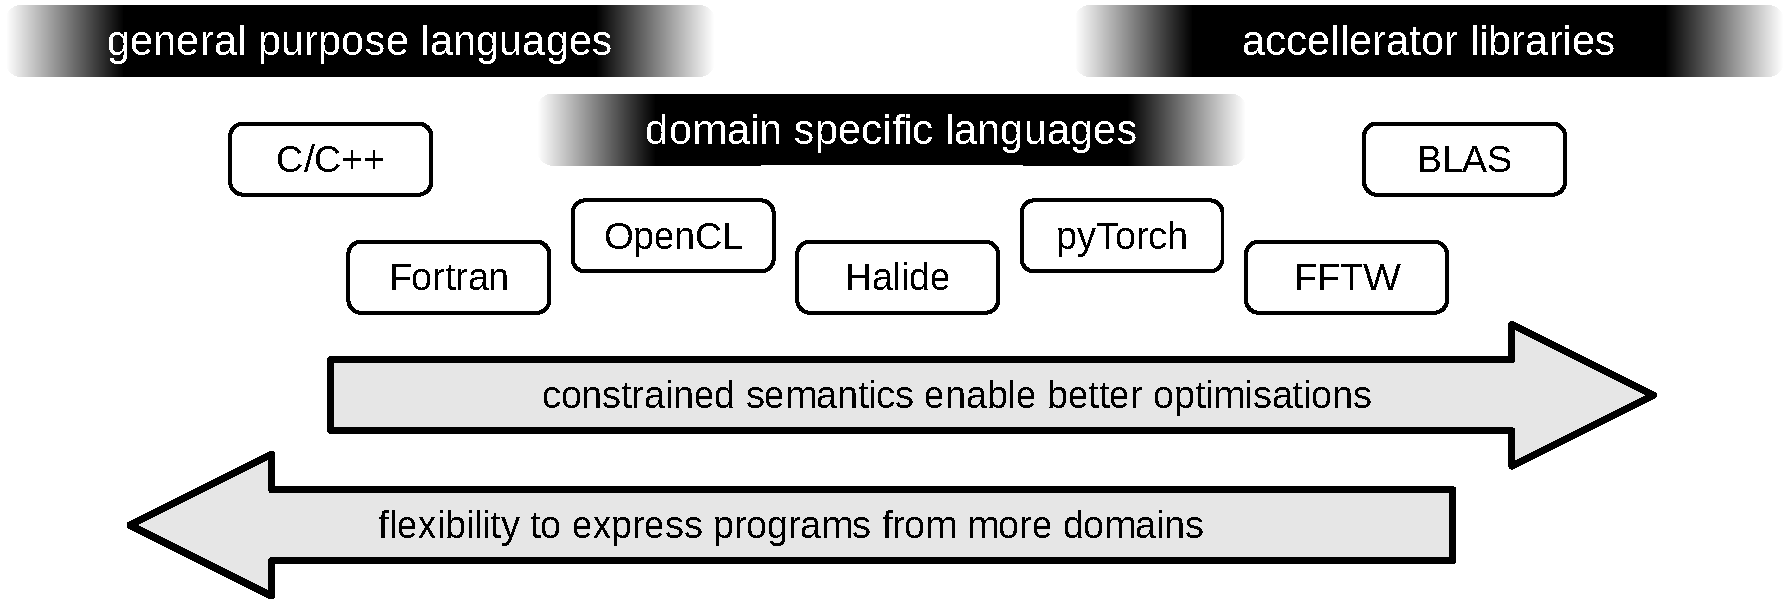
\includegraphics[width=\textwidth]{figures/DSLgradient}
\caption{Domain-specific languages on a spectrum between general-purpose
         languages and libraries:
         Less flexibility allows for stronger reasoning and greater
         optimisation potential.}
\label{specialgradient}
\end{figure}

    More broadly, the superior optimisation potential of libraries and
    kernel compilers is a consequence of operating under more constrained
    conditions than host compilers.
    While expert programmers can often apply domain knowledge themselves
    when using versatile general-purpose languages, this potential is
    uncovered automatically and tuned for the target hardware by specialised
    tools.
    The restrictions on input programs imply domain knowledge that is leveraged
    to make stronger assumptions, use more powerful reasoning and generate
    better code.

    {\bf Hypothesis:}\quad
    Restrictive program models expose additional optimisation
    opportunities and lead to increased portability.
    Compilers use program models that correspond closely to their input
    programming languages.
    This correspondence could be decoupled by recognising program parts that
    adhere to more constrained models, making the powerful domain-specific
    optimisation techniques of kernel compilers available to host compilers.

\section{Moving on the Spectrum of Specialisation}

    Host compilers need methods to automatically recognise restrictive program
    models within general-purpose code.
    The term {\it program model} in this context means an internal
    representation of program logic with corresponding reasoning and
    assumptions about the program semantics.
    Reformulating program sections in restrictive models would make the
    superior domain-specific reasoning from kernel compilers applicable in
    host compilers.
    This would result in a compiler that can combine the positive aspects of
    both sides of the spectrum of specialisation.

    Such an approach of detecting restricted models in general-purpose code has
    previously been used only for specific individual domains and required
    elaborate manually implemented compiler analysis functionality.
    For example, the Polly compiler by \citet{Lengauer2012Polly} takes
    arbitrary C/C++ code as input and recognises whether parts of this code
    are expressible in the more restrictive polyhedral model
    \citep{Karp:1967:OCU:321406.321418,benabderrahmane2010polyhedral}.
    The compiler reformulates the relevant code in this model, enabling
    advanced optimisation techniques that use the domain knowledge of the
    polyhedral model for generating faster code
    \citep{Moll:2016:ISS:2892208.2892217,Doerfert2015Polly}, substantiating the
    hypothesis.

\subsection{Contributions of this Thesis}

    This thesis derives a systematic and configurable method for recognising
    constrained program sections that fit restrictive models during the
    compilation process.
    The approach emerges from the analysis of a standard program model for
    host compilers: Static Single Assignment (SSA) form.
    Intermediate representations based on SSA are accessible to mathematical
    reasoning, with their most relevant features based on graph and list
    structures.
    With this in mind, structural restrictions on intermediate representation
    code -- corresponding to restricted domain-specific models -- can be
    precisely formulated as constraints on a mathematical characterisation of
    SSA form programs.
    Constraint solver techniques then make the automatic recognition of
    adhering code sections feasible.

    Instead of manually implementing sophisticated compiler analysis
    functionality, a flexible constraint programming language is introduced
    that can express many different such domain-specific models.
    An accompanying toolchain is developed that uses these specifications to
    automatically recognise code sections that satisfy them.
    This system captures the spectrum from \Cref{specialgradient}.
    On one extreme, sections of code are recognised as implementing
    specific algorithms, like matrix multiplications, that are parametrised with
    numeric values.
    Algorithms that allow parametrisation with an operator are next.
    Stencil kernels, reduction operations or generalised histogram computations
    fall into this category.
    More generic again are programs that merely follow certain structural
    restrictions, such as code adhering to the polyhedral model.
    \Cref{chapter:candl,chapter:reductions,chapter:idioms} cover each of these
    domains, culminating in a system for the automatic heterogeneous
    acceleration of sequential C/C++ code.

\section{Summary}

    The end of Moore's Law and Dennard Scaling has resulted in a shift away from
    homogeneous multi-processing, toward architectural innovation and
    specialised processor cores.
    The rising heterogeneity of computing resources poses a challenge to
    established compiler toolchains, which often only access the increasingly
    marginal homogeneous fraction of processing power.
    Therefore, programmers depend on domain-specific languages and libraries,
    which leverage domain knowledge from their restricted operating domains, to
    generate efficient code for this new hardware landscape.

    This domain knowledge can be made available to host compilers with
    approaches that automatically specialise general-purpose code and
    reformulate it in more restrictive program models.
    Previous work has established this on individual models, but this thesis
    develops a framework to formulate a wide range of restricted program models
    using a systematic approach based on constraint solving.
    To this purpose, a custom constraint programming language was developed
    and successively extended.
    Starting from a discussion of the underlying assumptions and features of
    Single Static Assignment code, the methodology is developed into a complete
    system, implemented as part of the mature Clang C/C++ compiler.

    In the later chapters, this core system is then applied in combination
    with other techniques in a range of different contexts.
    This includes the rapid prototyping of compiler optimisations, the
    automatic parallelisation of some program structures with indirect memory
    accesses, a new formulation of the polyhedral model and the detection of
    computational structures that cover important bottlenecks in typical
    scientific programs.

    Eventually, the techniques are combined into a fully integrated, extensible
    compiler tool for efficiently mapping sequential programs onto heterogeneous
    systems.
    This develops the thesis all the way from theoretical discussions of
    constraint programming approaches in compilers, to the experimental
    evaluation of real performance improvements on established benchmark suites
    and scientific applications.

\newpage
\section{Structure of the Thesis}

    This thesis is divided into six chapters.
    Following the introduction, the underlying methodology of this work is
    established in {\bf\Cref{chapter:theory}} and put in the context of
    conventional compiler analysis.
    Based on a model of Static Single Assignment (SSA) intermediate
    representations, the chapter derives a novel constraint programming approach
    to express algorithmic program structures as constraint formulas.
    Later sections of the chapter cover implementation decisions, algorithmic
    complexity, and a comparison to established Satisfiability Modulo Theory
    (SMT) problems.
    This forms the methodological basis for
    {\bf\Cref{chapter:candl,chapter:idioms,chapter:reductions}}.

    {\bf\Cref{chapter:literature}} gives a broad overview of the related work.
    This literature survey covers the four main areas of research in which this
    work is placed.
    Firstly, {\em constraint programming} underpins the methodology of this
    thesis.
    Secondly, {\em compiler analysis and auto-parallelisation} provide
    competing approaches against which the results in this thesis are evaluated.
    Thirdly, {\em heterogeneous computing} and the corresponding challenges
    motivate many of the compiler approaches that this research implements.
    Finally, ``{\em computational idiom}'' is an umbrella term for several
    overlapping concepts of algorithmic patterns that capture programming models
    in different positions on the spectrum of specialisation.

    {\bf\Cref{chapter:candl,chapter:idioms,chapter:reductions}}
    are each based on a published research article and elaborate on different
    applications of constraint programming in compilers.

    {\bf\Cref{chapter:candl}} develops a constraint programming language called
    CAnDL and presents an implementation in the LLVM compiler infrastructure.
    CAnDL specifications generate compiler analysis
    passes from declarative descriptions automatically via the CAnDL compiler.
    The chapter explores several compiler analysis tasks with CAnDL,
    including the implementation of peephole optimisations and the
    prototyping of graphics shader optimisations.
    This chapter is based on published research in
    \citet{Ginsbach:2018:CDS:3178372.3179515}.

    {\bf\Cref{chapter:reductions}} extends CAnDL into the Idiom Detection
    Langauge (IDL) and develops an auto-parallelising compiler for
    complex reduction and histogram computations built on IDL-powered analysis
    functionality.
    These computations cover many loops with indirect data access that are
    inaccessible to established approaches based on data flow and polyhedral
    analysis.
    The flexibility of constraint programming allows it to still capture such
    irregular computations.
    This chapter is based on published research in
    \citet{ginsbach2017discovery}.

    {\bf\Cref{chapter:idioms}} applies IDL to the detection of algorithmic
    structures that go beyond the scope of traditional compiler analysis:
    stencils, complex reductions and histograms, as well as sparse and dense
    forms of linear algebra.
    The detection in LLVM enables the automatic heterogeneous
    acceleration of sequential code and result in significant speedups on
    established benchmark suites.
    This chapter is based on published research in
    \citet{Ginsbach:2018:AML:3173162.3173182}.
